\documentclass[11pt]{article}

\usepackage[margin=1in]{geometry}
\usepackage{booktabs}
\usepackage{amsmath}
\usepackage{hyperref}
\usepackage{graphicx}
\usepackage{tikz}
\usetikzlibrary{arrows.meta, positioning, shapes.geometric}

\tikzset{
  flowbox/.style={
    rectangle,
    rounded corners,
    draw=black!65,
    fill=blue!5,
    align=center,
    text width=3.6cm,
    minimum height=1.0cm,
    font=\small
  },
  widebox/.style={
    rectangle,
    rounded corners,
    draw=black!65,
    fill=orange!8,
    align=center,
    text width=4.5cm,
    minimum height=1.0cm,
    font=\small
  },
  arrow/.style={-{Latex[length=2mm]}, thick}
}

\title{Football Corner Forecasting Report}
\author{Yujia Zhang \hfill 21 May 2026}
\date{}

\begin{document}
\maketitle

\section{Summary}

\quad \; The baseline appears to be a Poisson-style model using the 10 anonymised match
features plus the home indicator. This is a sensible starting point because
corners are non-negative counts.

The final model keeps this baseline structure and adds one new signal: a
pre-match estimate of each team's attacking strength from historical
corners. This signal is built with a Kalman filter, is strongly related to future
corners, and the correlations with the anonymised features are low.

Rows with too little team history or no history at all need a fallback. Instead of filling the
missing team-strength value with one global mean, a small regularised tree model
predicts that value from the available match features. This gives a steady and
reliable validation improvement.

More complex models and richer Kalman state splits were tested, but the dataset
is too small for them to be reliable, likely leading to overfits. The simpler Poisson model plus one clear
team-strength feature gave the best bias-variance tradeoff.

\section{Final Model and Validation Results}

The final model predicts the expected number of corners for each team in each
match. It uses the 10 anonymised match features, the home indicator, and one
extra team-strength feature: the team's estimated attacking corner strength
before the match.

The prediction model is a regularised Poisson GLM. Poisson is used because
corners are non-negative counts. ``Regularised'' means the model is discouraged
from using very large coefficients, which helps avoid overfitting.
\[
\hat{y} \sim \texttt{PoissonRegressor}(\alpha=0.1).
\]

The value \(\alpha=0.1\) is the L2 penalty strength, selected on the tune seasons not on the validation seasons. The objective it minimises is:
\[
\text{Poisson count loss} + 0.1 \times \text{coefficient penalty}.
\]
The best model is chosen as the one with the lowest loss:
\[
0.25 \times \text{MAE}
+ 0.25 \times \text{RMSE}
+ 0.50 \times \text{Poisson deviance}.
\]
The loss is the combination of three metrics that check different aspects of corner prediction quality.
Poisson deviance receives the largest weight because corners are count data, so
the model should generally fit the shape of a count outcome, not only minimise ordinary
distance errors. MAE and RMSE are still included because the submitted output is
a point prediction: MAE measures the typical miss in corners, while RMSE gives
extra punishment to large misses.

The final table compares three models. The baseline is the provided reference
prediction. The second row adds the Kalman attack-strength feature but fills
missing values with a simple mean. The third row is the final model: when team
history is insufficient, it uses a small tree model to estimate the missing
attack-strength value instead of using one global mean. Lower is better for all
three metrics.

\begin{table}[h]
\centering
\begin{tabular}{lrrr}
\toprule
Model & MAE & RMSE & Poisson deviance \\
\midrule
Baseline & 2.2717 & 2.8574 & 1.3406 \\
Poisson + mean-filled Kalman attack feature & 2.1712 & 2.7349 & 1.2574 \\
Poisson + cold-start Kalman attack prior & 2.1588 & 2.7196 & 1.2437 \\
\bottomrule
\end{tabular}
\end{table}

\section{Reproducing the Results}

\subsection{Dependencies}

The code requires Python 3.10 or later with the following packages:

\begin{verbatim}
numpy pandas scikit-learn
\end{verbatim}

The code also uses the standard library modules \texttt{collections},
\texttt{dataclasses}, and \texttt{pathlib}, which are included with Python.


\subsection{Generating holdout predictions}

Data exploration is in \texttt{data\_exploration.ipynb}.
The full modelling workflow---Kalman filter design, hyperparameter search,
ablation grid, cold-start prior comparison, and one-shot validation---is
documented in
\texttt{Kalman\_filter\_based\_team\_strength.ipynb}.
The final prediction pipeline is in \texttt{predict.py}; run the following command from the project root:

\begin{verbatim}
python predict.py
\end{verbatim}

The script trains the final Poisson model on all labelled seasons (2012--2022),
applies the Kalman filter and cold-start prior to both the training and holdout
rows, and writes the output file.

\subsection{Output file}

The predictions are written to:

\begin{verbatim}
outputs/predictions.csv
\end{verbatim}

The file contains one row per (match, team). Its columns are:
\begin{verbatim}
match_id, team, predicted_corners
\end{verbatim}

\section{Train-tune-validation Periods}

All model choices are made before the final validation period:
\[
\text{CORE}=2012\text{-}2017,\quad \text{TUNE}=2018\text{-}2019.
\]
The final one-shot check is:
\[
\text{TRAIN}=2012\text{-}2019,\quad \text{VAL}=2020\text{-}2022.
\]

During validation feature construction, validation corners are masked before the
Kalman filter is run. This means validation rows can receive pre-match states,
but they cannot update any hidden state or home-advantage estimate.

\section{Kalman Filter Team Strength}

\subsection{How the filter works}

Each team has two hidden states:
\[
\text{attack}_t = \text{corners the team tends to win},
\]
\[
\text{defense}_t = \text{corners the team tends to allow the opponent to win}.
\]

\begin{figure}[h]
\centering
\resizebox{\textwidth}{!}{%
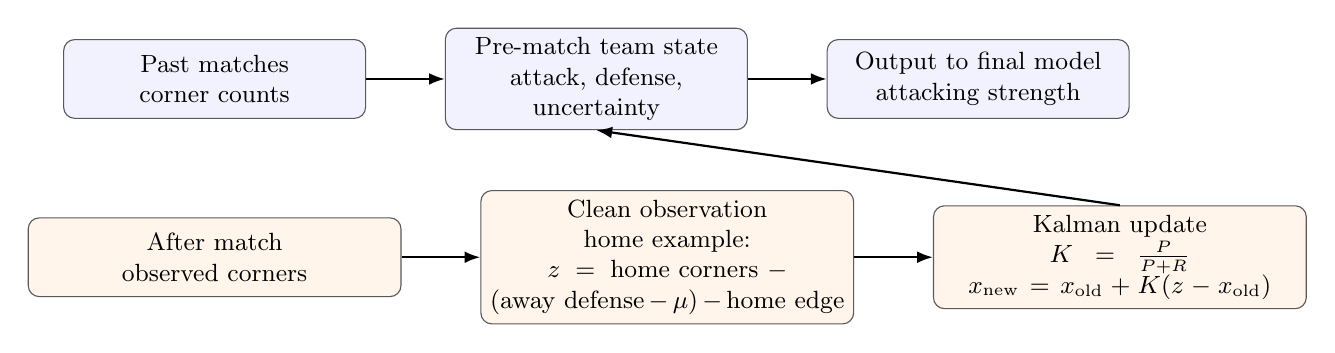
\begin{tikzpicture}[node distance=1.2cm and 1.0cm]
  \node[flowbox] (past) {Past matches\\corner counts};
  \node[flowbox, right=of past] (state) {Pre-match team state\\attack, defense, uncertainty};
  \node[flowbox, right=of state] (feature) {Output to final model\\attacking strength};

  \node[widebox, below=1.25cm of past] (obs) {After match\\observed corners};
  \node[widebox, right=of obs] (clean) {Clean observation\\home example:\\\(z=\text{home corners}-(\text{away defense}-\mu)-\text{home edge}\)};
  \node[widebox, right=of clean] (update) {Kalman update\\\(K=\frac{P}{P+R}\)\\\(x_{\text{new}}=x_{\text{old}}+K(z-x_{\text{old}})\)};

  \draw[arrow] (past) -- (state);
  \draw[arrow] (state) -- (feature);
  \draw[arrow] (obs) -- (clean);
  \draw[arrow] (clean) -- (update);
  \draw[arrow] (update.north) -- (state.south);
\end{tikzpicture}
}
\caption{Kalman filter flow. The filter keeps one simple attacking signal for
the final predictor; defence is used only to clean the update signal.}
\end{figure}

Raw corners are not a pure attack signal. A simple way to read a home team's
corner count is:
\[
\text{home corners}
\approx
\text{home attack}
+(\text{away defense}-\text{league mean})
+\text{home advantage}.
\]
So before updating home attack, the filter subtracts the current opponent
defense estimate and the league home advantage:
\[
z_{\text{home attack}}
=
\text{home corners}
-(\text{away defense}-\mu)
-\text{home advantage}.
\]
Here \(\mu\) is the league-average corner level. If the away defense estimate
equals the league mean it adds no adjustment; if it is above the mean that team
allows extra opponent corners, and only that excess is removed from the raw home
count. The same idea applies to away attack and to both defense states.

For each hidden state the Kalman update is:
\[
K = \frac{P}{P+R},
\qquad
x_{\text{new}} = x_{\text{old}} + K(z-x_{\text{old}}),
\qquad
P_{\text{new}} = (1-K)P.
\]
If the state is uncertain, the new match is trusted more; if the match
observation is noisy, the update is more conservative.

Matches on the same date are batched: all pre-match features for that date are
recorded first, then all hidden states are updated together. This avoids
same-day leakage where an early kick-off could otherwise affect a later
kick-off's features.

\subsection{Why not a richer state space}

The retained design keeps one attacking state and one defensive state per team,
with home advantage handled as a league-level constant. A richer design was
also tested, splitting each state into separate home and away versions: home
attack, away attack, home defense, away defense. Conceptually this is
attractive because teams can behave differently at home and away.

\begin{figure}[h]
\centering
\resizebox{\textwidth}{!}{%
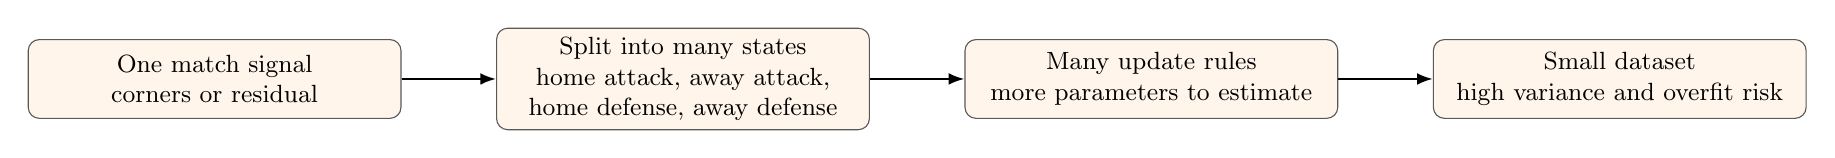
\begin{tikzpicture}[node distance=1.0cm and 1.2cm]
  \node[widebox] (input) {One match signal\\corners or residual};
  \node[widebox, right=of input] (split) {Split into many states\\home attack, away attack, home defense, away defense};
  \node[widebox, right=of split] (update) {Many update rules\\more parameters to estimate};
  \node[widebox, right=of update] (risk) {Small dataset\\high variance and overfit risk};

  \draw[arrow] (input) -- (split);
  \draw[arrow] (split) -- (update);
  \draw[arrow] (update) -- (risk);
\end{tikzpicture}
}
\caption{Richer Kalman design tested but not retained. More expressive, but
it spreads the limited data across too many hidden states.}
\end{figure}

The cost is that each team now needs four hidden states instead of two, so each
state receives fewer effective observations. With only 40 teams and 11 seasons
the richer version had higher variance: it explained past data in more detail,
but those details were not stable enough to improve future predictions. The
simpler design is a better bias-variance tradeoff for this dataset.

\subsection{Why not Elo-style ratings}

An Elo-style model was also considered. Elo works well when one scalar rating
can be updated from one match result. Corner prediction needs more structure:
attacking strength, defensive weakness, home effect, and away effect. A
multi-rating Elo would therefore require separate home attack, away attack,
home defense, and away defense parameters per team, plus manual choices for the
initial rating, update rates, home adjustment, and mean-reversion speed. With
this dataset there is not enough validation data to tune all those choices
reliably.

The Kalman filter handles updates more automatically. It tracks both an
estimate and an uncertainty for each hidden state, so uncertain teams update
more and stable teams update less. It requires only two hyperparameters
(process noise and observation noise), both of which were selected on the tune
period with a simple grid search.

\subsection{Which Kalman signal to use}

The filter exposes four pre-match signals per row: own attacking strength, own
defensive weakness, opponent attacking strength, and opponent defensive
weakness. Only the team's own attacking strength is used in the final model.
This was not chosen by intuition alone; it was verified empirically.

\begin{table}[h]
\centering
\begin{tabular}{lr}
\toprule
Kalman signal & Correlation with corners \\
\midrule
Own attacking strength & 0.2731 \\
Own defensive weakness & -0.0145 \\
Opponent attacking strength & -0.0152 \\
Opponent defensive weakness & -0.0129 \\
\bottomrule
\end{tabular}
\caption{Correlation on training rows after the Kalman warm-up period. Only
the attacking-strength signal has a clear direct relationship to the target.}
\end{table}

The attacking-strength signal is also not a duplicate of the 10 anonymised
match features: its average absolute correlation with those features is 0.127
and the largest is 0.326, so it adds team-history information not already
contained in the anonymised inputs.

\begin{table}[h]
\centering
\begin{tabular}{lrrr}
\toprule
Tune-period model & MAE & RMSE & Poisson deviance \\
\midrule
No Kalman feature & 2.1683 & 2.6954 & 1.3753 \\
Add own attacking strength & 2.1399 & 2.6496 & 1.3379 \\
Add attacking and defensive strength & 2.1404 & 2.6498 & 1.3380 \\
Add all four Kalman signals & 2.1465 & 2.6575 & 1.3439 \\
\bottomrule
\end{tabular}
\caption{Tune-period ablation for Kalman feature selection. Adding the
attacking-strength signal improves the model; adding the other signals does
not improve it further.}
\end{table}

One additional Kalman feature gives a clear tune-period gain, while adding the
remaining signals introduces complexity without a robust improvement.

\section{Cold-Start Prior}

\subsection{Why the problem is significant}

The Kalman filter requires a warm-up period before its estimates are reliable.
A pre-match attacking-strength estimate is only recorded once \emph{both} the
team and its opponent have each completed at least 5 earlier matches. This is
intentional: without enough history, the Kalman state is mostly just its prior
mean rather than learned team information.

The issue matters in this dataset. In the labelled history used for the final
training run, 185 matches (370 team rows, 8.9\,\% of labelled rows) do not yet
have a usable Kalman attack estimate. The holdout set has a larger cold-start
problem. Four of the 28 holdout teams, \texttt{team\_30}, \texttt{team\_34},
\texttt{team\_36}, and \texttt{team\_47}, never appear in the labelled data at
all, covering 190 holdout team rows. Because the filter requires both teams in
a match to have enough history, these new teams also affect their opponents'
rows. In total, \textbf{360 of the 1{,}520 holdout rows (23.7\,\%) have no
usable pre-match attack estimate before filling.}

\subsection{Why a global mean is not enough}

A global-mean fill would assign every cold-start team the same average
attack strength, ignoring all 10 anonymised match features and the home
indicator. For a completely new team, those features are the only signal
about how corner-prone it is likely to be.
Different teams have different feature profiles and plausibly different
attacking strengths; collapsing them to one number discards that signal.

\subsection{What the prior model does}

The prior is not a second corner-count model. It only estimates the missing
Kalman attack-strength value. It is trained on historical rows where the
Kalman filter has already produced a real pre-match attack estimate, using the
available row-level information:
\[
(\text{10 anonymised match features},\;\text{home indicator})
\;\longrightarrow\;
\text{Kalman attack-strength estimate}.
\]
At prediction time, rows with real Kalman history keep their original attack
estimate untouched. Only missing values are filled by the prior. The final
Poisson model then sees the same kind of input for every row: the 10 anonymised
features, the home indicator, and one attack-strength estimate. That estimate
comes from real Kalman history where possible, and from the prior only when
history is missing.

\subsection{Conservative clipping}

After the prior produces an initial attack value, that value is clipped to the
5th--95th percentile of real Kalman attack estimates observed in training.
This prevents the prior from assigning implausibly large or small values for
feature combinations it has not seen. The prior can still distinguish stronger
from weaker cold-start rows within that range; it simply cannot extrapolate to
an extreme initial strength unsupported by the historical states.


\subsection{Model choice and hyperparameters}

Ridge regression and \texttt{HistGradientBoostingRegressor} were both tested
as the prior model on the tune period.
Ridge assumes a linear relationship between the anonymised features and
the Kalman attack estimate; it also requires the features to be on comparable
scales, which cannot be verified for anonymous inputs.
\texttt{HistGradientBoostingRegressor} (HGB) makes neither assumption: it can
capture non-linear feature-to-attack relationships and handles mixed-scale
inputs natively without preprocessing.

\begin{table}[h]
\centering
\begin{tabular}{lrrr}
\toprule
Prior model & MAE & RMSE & Poisson deviance \\
\midrule
Ridge ($\alpha=1$)   & 2.1522 & 2.6765 & 1.3552 \\
Ridge ($\alpha=10$)  & 2.1533 & 2.6779 & 1.3564 \\
Ridge ($\alpha=100$) & 2.1583 & 2.6849 & 1.3623 \\
HGB (selected)       & 2.1460 & 2.6685 & 1.3503 \\
\bottomrule
\end{tabular}
\caption{Tune-period comparison of cold-start prior models, evaluated on all
tune rows including cold-start rows. HGB outperforms the best Ridge variant
on every metric.}
\end{table}

HGB outperforms the best Ridge variant on every metric.
\texttt{HistGradientBoostingRegressor} is therefore used because it handles
mixed-scale anonymous features without manual preprocessing and can capture
non-linear relationships between the features and attack strength.

The parameters are set to be deliberately conservative rather than
aggressively optimised:

\begin{table}[h]
\centering
\begin{tabular}{llp{6.5cm}}
\toprule
Parameter & Value & Reason \\
\midrule
\texttt{max\_iter}         & 100  & Limits ensemble size \\
\texttt{max\_leaf\_nodes}  & 15   & Keeps individual trees small and shallow \\
\texttt{min\_samples\_leaf}& 30   & Roughly 1\,\% of training rows per leaf \\
\texttt{l2\_regularization}& 5.0  & Strong weight shrinkage \\
\texttt{learning\_rate}    & 0.03 & Slow, stable updates \\
\bottomrule
\end{tabular}
\caption{Cold-start prior hyperparameters. All settings favour stability over
fitting power, because the prior is a fallback rather than the main model.}
\end{table}

The hyperparameters were set by hand to produce stable, non-extreme estimates.
Aggressive tuning would risk overfitting the features-to-attack mapping on a
relatively small training set, which would defeat the purpose of being
conservative. The benefit of the prior over a plain mean fill was confirmed
on the tune period before the validation period was touched:
mean-fill gave a tune MAE of 2.1638, while the prior-fill gave 2.1460.
The same ordering held on the one-shot validation check (MAE 2.1712
versus 2.1588).

\subsection{Pipeline integration}

In the final prediction pipeline the Kalman filter is first run over all
labelled rows concatenated with the holdout rows. Labelled rows update the
hidden states; holdout rows receive pre-match states but do not update
anything because their corners are unknown. The Poisson corner model is fitted
only on labelled rows that have real Kalman history. The cold-start prior is
then fitted on those same rows and applied to fill missing attack-strength
values in the holdout. The prior is therefore used only as a targeted fallback
for missing team-history information, not as a replacement for either the
Kalman filter or the final corner model.


\section{Removed Experiments}

Each experiment below was evaluated on the tune period under the same criteria. None improved the result robustly; the reasons
fall into three categories.

\subsection{Redundant signal: already captured by existing features}

\paragraph{Static team target encoding.}
Each team's historical mean corners scored and conceded were added as extra
features. These are cruder versions of the Kalman attack-strength feature: the
filter already summarises each team's attacking history, updating that estimate
match by match with uncertainty tracking. The static mean ignores recency and
carries no uncertainty signal. In ablation it added nothing after the Kalman
attack feature was already in the model.

\paragraph{Rolling form features.}
Short-window rolling means (last 3, 5, and 10 matches) overlap substantially
with what the Kalman attack feature already captures. The Kalman filter is
itself a weighted average of past observations, emphasising recent matches
through its uncertainty dynamics. Adding rolling means alongside it therefore
introduces near-duplicate columns. The tune-period ablation showed no
consistent gain from any rolling window, alone or combined with the Kalman
attack feature.

\paragraph{Team, opponent, and season identity features.}
Team and opponent identities are already represented through the Kalman attack
feature. Adding them as categorical dummy variables asks the model to re-learn
a static per-team offset that the Kalman feature already provides dynamically.
Season identity produced a scale problem: the raw year values (2012--2022) are
an order of magnitude larger than the other features, which destabilised the
Poisson GLM and caused convergence issues even after regularisation.

\paragraph{Frozen home/away drift features.}
Separate home-only and away-only rolling averages were considered to capture
venue-specific form. After controlling for the \texttt{home} indicator and
the Kalman attack feature, the residual home/away drift signal was too small
to recover reliably in the tune period.

\subsection{Too many parameters for the dataset size}

The training set contains around 4{,}180 rows (2{,}090 matches $\times$ 2
rows). Any model that introduces many new parameters to estimate risks high
variance: it can fit the training data well but generalises poorly.

\paragraph{Rich Kalman filter with separate home and away states.}
The simpler Kalman design keeps two states per team (attack and defence).
A richer version was also tested that splits each into a home and an away
state, giving four states per team. With 40 teams this means roughly 160
latent variables to track instead of 80. Each state receives fewer effective
observations, so the estimates are noisier. The richer design produced a
worse honest validation result (VAL MAE\,2.276 versus 2.159) despite being
more expressive in principle.

\paragraph{Tree models, random forest, GBM, and XGBoost as the main corner model.}
Non-linear tree ensembles were tested with a Poisson or Tweedie objective.
With only around 4{,}000 training rows, these models need strong regularisation
and careful cross-validation to avoid overfitting. Even with early stopping and
depth limits, none improved reliably over the simple Poisson GLM on the tune
period. The anonymised features also provide no natural interaction structure
to exploit, so the non-linear capacity was not needed.

\paragraph{Semi-linear and GAM-style Poisson models.}
Generalised additive models allow some features to enter through smooth spline
terms rather than linearly. Each spline term adds effective degrees of freedom.
With the current feature set and dataset size, this extra flexibility did not
help: the spline fits on CORE generalised poorly to TUNE.

\paragraph{Tweedie and Negative Binomial GLMs.}
Corner counts show genuine overdispersion: the marginal variance-to-mean ratio
is approximately 1.84, which in principle motivates a Tweedie or Negative
Binomial distribution over plain Poisson. Despite this theoretical motivation,
neither improved over Poisson on the tune period. Three factors explain why.

First, each model introduces one additional global parameter to estimate
alongside the regularisation strength: the power $p\in(1,2)$ for Tweedie, or
the dispersion $\phi$ for Negative Binomial. Tuning two coupled parameters
reliably requires more data than the roughly 4{,}000 training rows provide.

Second, the marginal variance-to-mean ratio of 1.84 reflects
between-team heterogeneity---strong attacking teams consistently win more
corners. This source of overdispersion is already handled by the team-strength
feature from the Kalman filter. The residual overdispersion after conditioning
on all features is likely considerably smaller than the marginal figure.

Third, the composite tuning metric weights Poisson deviance most heavily.
Tweedie and Negative Binomial models are optimised under their own likelihoods,
which are not the same criterion. Even a distributional improvement can go
undetected if the chosen evaluation measure is calibrated to Poisson.


\section{What Next}

Four directions below

\subsection{Non-linear team-strength response}

The Poisson GLM assumes a log-linear relationship between the attacking-strength
feature and expected corners. This may be too rigid: a team whose attack
estimate is far above average might produce corners at a rate that grows faster
than the linear term implies. A Poisson GAM with a smooth spline on the
attacking-strength feature and linear terms for the base features would test
whether a non-linear response adds predictive value. 

\subsection{Season-boundary state decay}

The Kalman filter currently carries team states unchanged from the last match of
one season to the first match of the next. Teams change substantially over a
summer: new signings, departures, new manager, pre-season form. Shrinking each
state towards the league mean at each season boundary---with a tunable decay
parameter---would better reflect this turnover. 


\subsection{Opponent-aware cold-start prior}

The current prior predicts a team's attacking strength from its own match
features only. When the prior is applied, the opponent's Kalman attack and
defence estimates are often already available. Adding those as inputs to the
prior would make cold-start estimates sensitive to match context: a new team
playing a historically strong defensive side should receive a lower initial
attacking estimate than the same team playing a weak one.

\subsection{Rolling cross-validation for hyperparameters}

The process-noise and observation-noise grid search and the regularisation sweep
both rely on a single CORE to TUNE split. Rolling-window cross-validation---for
example training on 2012--2015 and predicting 2016--2017, then shifting the
window forward by two years---would give more robust hyperparameter estimates
and reduce the risk that the selected values happen to fit one particular
two-year tune period well.

\end{document}
